\documentclass[11pt, a4paper]{article}

\usepackage{graphicx}
\usepackage[a4paper,top=3cm,bottom=2cm,left=2cm,right=2cm,marginparwidth=1.75cm]{geometry}
\usepackage[english]{babel}
\usepackage[utf8x]{inputenc}
\usepackage{subfig}
\usepackage{amsmath}
\usepackage{amssymb}

\graphicspath{ {./images} }
\newcommand*{\qed}{\hfill\ensuremath{\quad\square}}%
\newcommand*{\rad}{\ensuremath{\,\text{rad}}}
\newcommand*{\R}{\ensuremath{\mathbb{R}}}

\makeatletter
\renewcommand*\env@matrix[1][*\c@MaxMatrixCols c]{%
  \hskip -\arraycolsep
  \let\@ifnextchar\new@ifnextchar
  \array{#1}}
\makeatother

\newtheorem{theorem}{Theorem}

%------------------------------------------------
%Templates for images and figures
% \begin{figure}[h]
%   \centering
%   \subfloat[caption 1]{{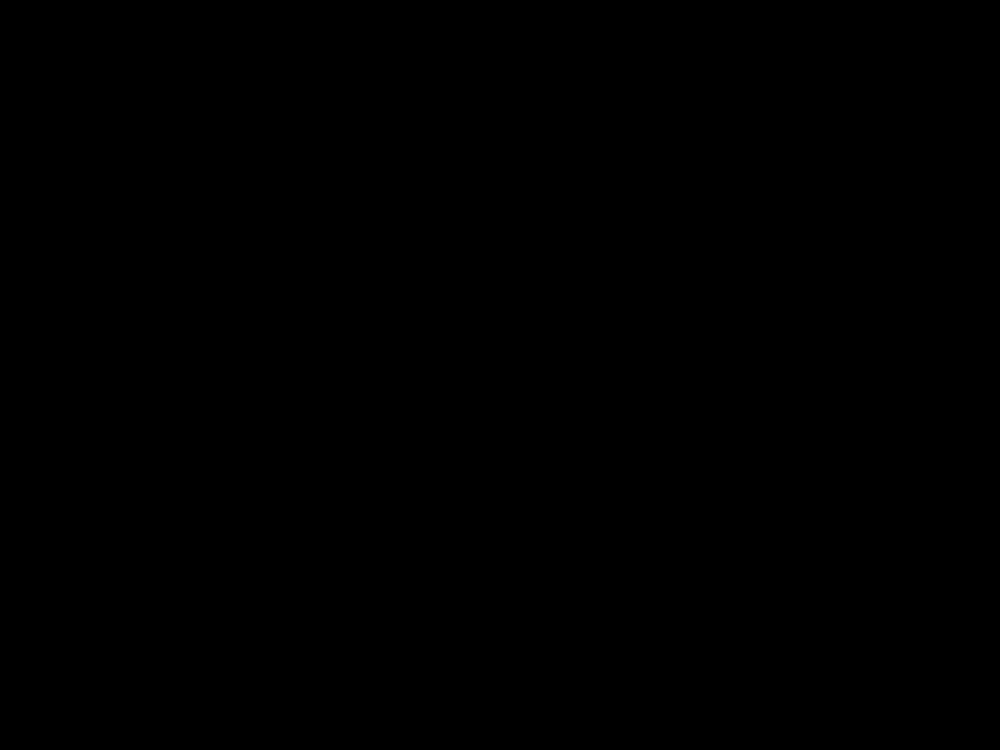
\includegraphics[width=30mm]{images/placeholder.png}}}%
%   \qquad
%   \subfloat[caption 2]{{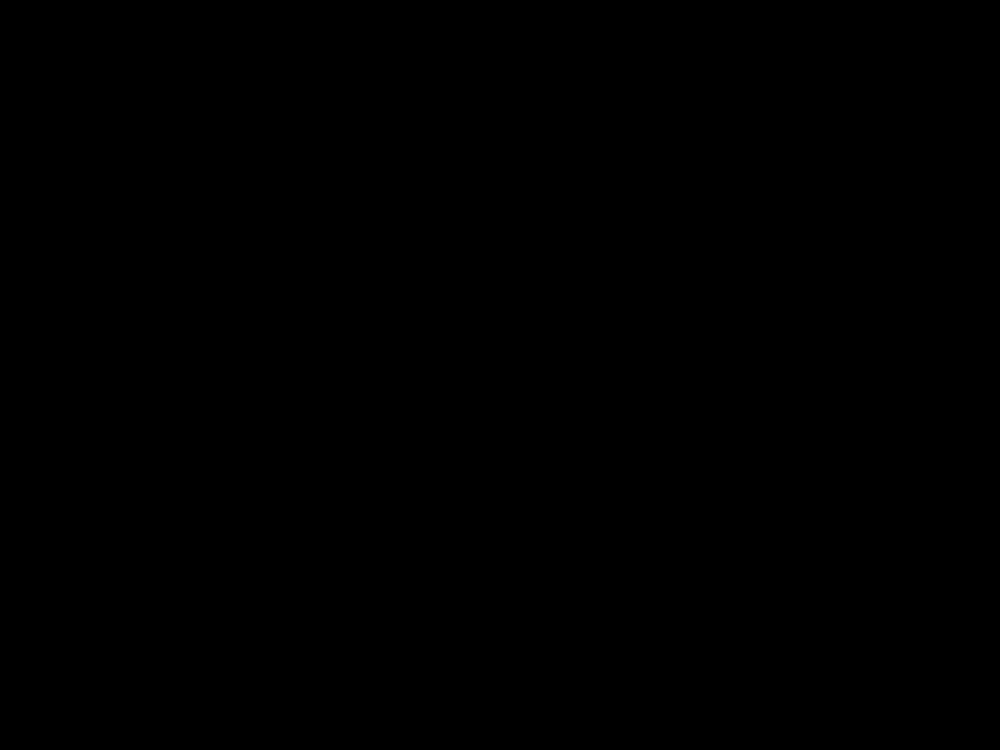
\includegraphics[width=30mm]{images/placeholder.png}}}%
%   \caption{Description}
% \end{figure}

% \begin{figure}[h]
%   \centerline{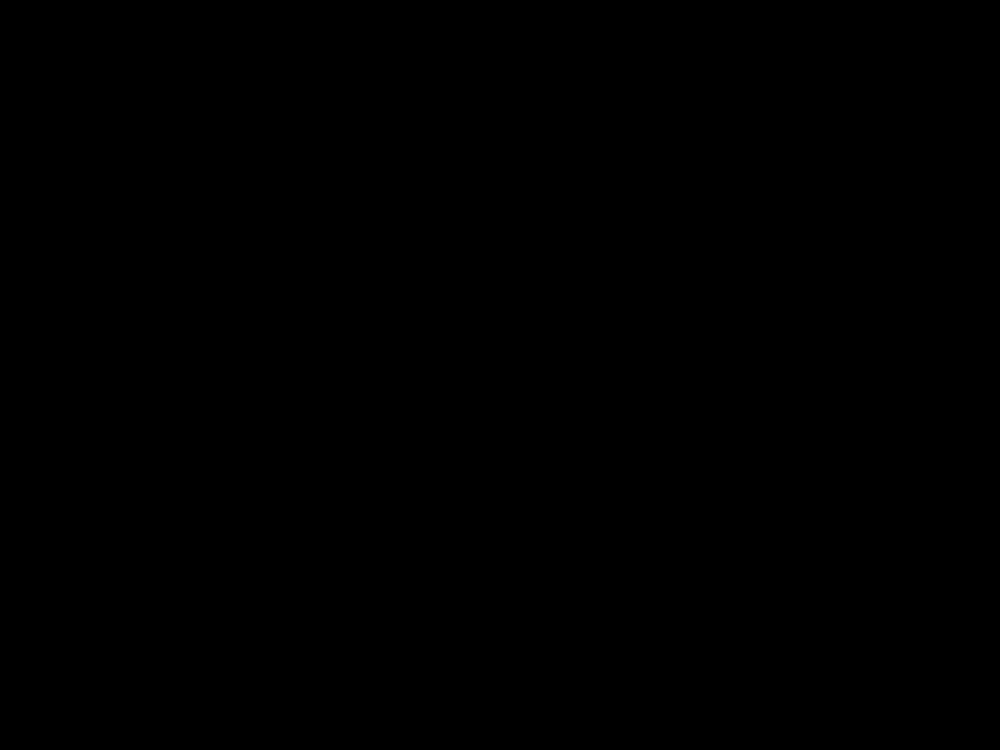
\includegraphics[width=50mm]{images/placeholder.png}}
%   \caption{Description}
% \end{figure}
%-----------------------------------------------

\begin{document}
\setcounter{section}{3}
\setcounter{equation}{0}
\section{Thermofluids Lecture 4: Thermodynamic states (30/04/2020)}


\subsection{State principle for simple compressible systems}
The value of 2 independent properties determin the values of all other intensive propeties of a system. These 2 independent properties can be used in a diagram to determine the phase of a given substance. The most common combination of variables for these type diagrams are $(T, v)$ and $(p, v)$. Where $T$ is temperature, $p$ pressure and $v$ specific volume. Note that pressure and temperature aren't always 2 independent sets of varibales (like in a 2-phase region). To illustrate what it means for 2 variables to be dependent consider the following variables $(v, \rho)$:
\begin{gather}
  v = \frac{V}{m}\\
  \rho = \frac{m}{V} = \frac{1}{v}
\end{gather}
Thus since there is a direct relation between the specific volume $v$ and the density $\rho$ these variables are considered to be dependen on eachother. Another point of note is that the variables used to express the state of a system cannot depend on an randomly chosen datum. This excludes properties like height and velocity.


\subsection{$(T, v)$-diagrams}
The thermodynamic state of a system can be changed by either adding work or heat. The easiest example of state diagrams is the $(T, v)$-diagram of water. The diagram of water at an arbitrary pressure $p$ which is smaller the critical pressure $p_{crit}$ can be found in figure 1.
\begin{figure}[h]
  \centerline{\includegraphics[width=60mm]{images/water process.png}}
  \caption{The $(T, v)$-diagram of the process of heating water at an arbitrary subcritical constant pressure.}
\end{figure}
\begin{enumerate}
  \item compressed liquid, A the temperature increases there is a small increase in volume as the kinetic energy of molecules increases.
  \item Saturated liquid, the point at which the water is just about to vaporize
  \item Saturated liquid-vapor mixture, Liquid and vapor coexist in equilibrium. The temperature $T$ stops increasing since all added heat is used for vaporizing the water. $v$ does keep increasing since vapor has a higher specific volume then water and the amount of vapor is steadily increasing.
  \item Saturated vapor, The vapor is about to condense.
  \item Superheated vapor, All vapor which expands when more heat is added.
\end{enumerate}
Note that the trajectory of water in figure 1 is dependent on the pressure $p$. Since we are only considering changes in the specific volume and temperature the pressure is assumed to be constant. When the line in the diagram is drawn again at a different, higher pressure $p$ it can be seen that the water stays a compressed liquid at higher temperatures. Doing this a couple more times and plotting them all in the same figure would result in a curve which is shown if figure 2. 
\begin{figure}[h]
  \centerline{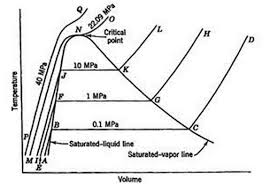
\includegraphics[width=80mm]{images/T,v diagram.jpg}}
  \caption{The curve revealing the Saturated liquid line, saturated vapor line and the critical point (source: https://web.mit.edu/16.unified/www/FALL/thermodynamics/notes/node61.html)}
\end{figure}
Note that if the pressure is high enough (read equal to or higher then the critical pressure) the water will not transition from liquid to vapor. At this pressure saturated liquid and vapor are considered to be indetical and phase boundaries just vanish. The critical point is defined by a critical temperature $T_c$ and a critical pressure $p_{crit}$. $T_c$ can be thought of as the maximum temperature at which it is possible for a liquid and vapor to coexist in equilibrium.


\subsection{$(p, v)$-diagrams}
The $(p, v)$-diagram shows the relation between the pressure and specfic volume of a substance. Note that the curve for this relation looks alot like the curve in the $(T, v)$-diagram.
\begin{figure}[h]
  \centerline{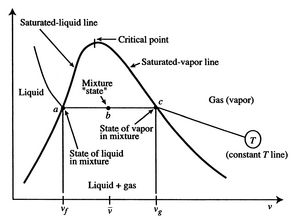
\includegraphics[width=80mm]{images/p,v diagram.jpg}}
  \caption{The $(p, v)$-diagram of a pure substance, found by repeating the same process of the $(T, v)$-diagram. (source: https://web.mit.edu/16.unified/www/FALL/thermodynamics/notes/node61.html)}
\end{figure}
The diagram in figure 3 can be extended to include the solid, solid-liquid and solid-vapor states. This leaves us with 2 types of diagram. 1 for substances which contract when they solidify\footnote{Freezing when we talk about water} (most substances) and substances which expand when they solidify (water, bismuth, plutonium).
\begin{figure}[h]
  \centering
  \subfloat[contracts on freezing]{{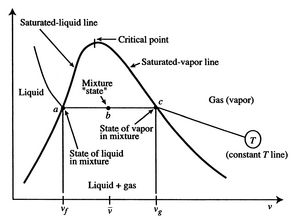
\includegraphics[width=60mm]{images/p,v diagram.png}}}%
  \qquad \qquad \qquad 
  \subfloat[expands on freezing]{{\includegraphics[width=60mm]{images/p,v diagram (water).png}}}%
  \caption{The complete $(p, v)$-diagram including the solid state}
\end{figure}
Note the straight line labeled Triple line at the bottom. This line labels the conditions for which all three phases of a pure substance coexist in equilibrium. The triple line apears as a single point on a $(p, T)$-diagram and thus is often also referred to as the triple point. An example of a triple point is water with $T=0.01\, ^\circ C$ and $p=0.6117\,kPa$. When precisly these values are met the solid, liquid and vapor state of water all coexist in equilibrium.


\subsection{$(p,T)$-diagrams}
The $(p, T)$-diagram, often also called the phase diagram, is a diagram which represent the phase of a pure substance for any random combination of pressure and temperature. The lines seperate the different phases. Note that the vaporization line stops at the critical point since there can be made no distinction between liquid and vapor above this point.
\begin{figure}[h]
  \centerline{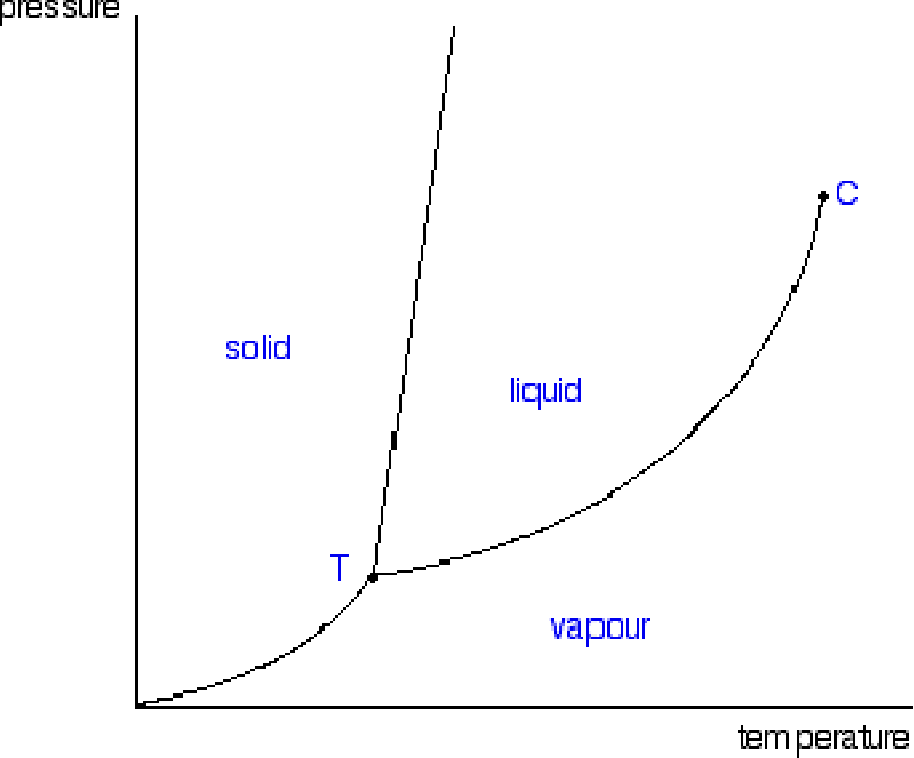
\includegraphics[width=60mm]{images/p,T diagram.png}}
  \caption{The $(p, T)$-diagram (sometimes called a phasediagram) of a pure substance (source: https://www.chemguide.co.uk/physical/phaseeqia/phasediags.html)}
\end{figure}


\subsection{$(p,v,T)$-surfaces}
Sometimes the $()$-diagram and $()$-diagram are combined into 1 big surface plot which relates the temperature, pressure and specific volume of a pure substance in 1 surface plot. This surface plot can be viewed as a multivariable function of the form $z=f(x, y)$. This means that the 2 variables $x, y$, which can be either $p$, $v$ or $T$, completely fix the state of a substance. Once these 2 variables are fixed all the other properties become dependent properties. The most conventional variation of this plot is the $(p, v, T)$-surface where $p = p(v, T)$.
\begin{figure}[h]
  \centering
  \subfloat[$(p, v, T)$-surface for a substance which expands on solidification]{{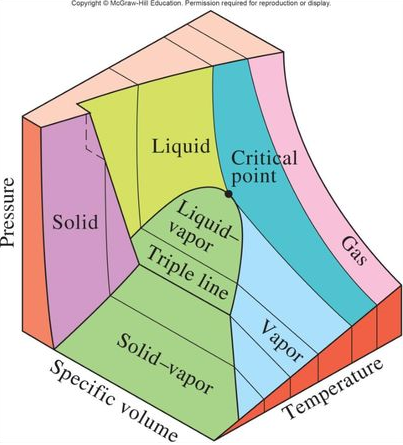
\includegraphics[width=40mm]{images/p,v,T surface (water).png}}}%
  \qquad \qquad \qquad 
  \subfloat[$(p, v, T)$-surface for a substance which contracts on solidification]{{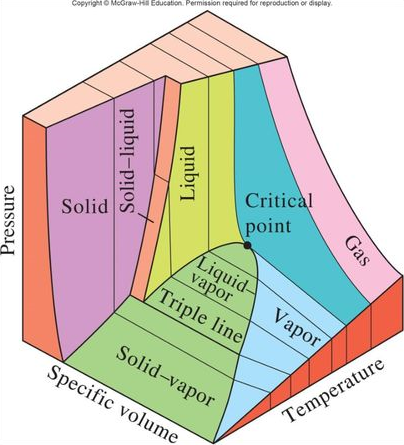
\includegraphics[width=40mm]{images/p,v,T surface.png}}}%
  \caption{The $(p, v, T)$-surface diagram (Source: Thermodynamics an engineering aproach)}
\end{figure}


\subsection{2-phase mixtures}
When vapor is created the pressure and temperature stay constant. Because of this it's not possible to use $(p, T)$-diagrams, since $p$ and $T$ are no longer independent variables. For a 2-phase mixture liquid-vapor mixture the ratio of mass and total mass represents the quality denoted as $x$. The value ranges from $0$ to $1$ where $0$ represents all saturated liquid and $1$ represents all saturated vapor. Since mass needs to be conserved we know the following:
\begin{equation}
  m_{t} = m_g + m_l
\end{equation}
The quality of a mixture is then given by the following equation:
\begin{equation}
  x = \frac{m_g}{m_{t}}
\end{equation}
Because we know that the total volume doesn't change (extensive property):
\begin{gather}
  V_{t} = V_l + V_g
  m_{t}v_{t} = m_lv_l + m_gv_g
\end{gather}
Which gives the following relation:
\begin{equation}
  v_t = \frac{m_l}{m_{t}}v_l + \frac{m_g}{m_{t}} v_g = (1 - x)v_l + xv_g
\end{equation}


\end{document}